\subsection{Teleoperation \& telepresence}
\frame
{
  \frametitle{Teleoperation \& telepresence}
  
  \emph{We need the equivalent of a body in a remote environment,
    with which we can move around, perform the proper actions through,
    observe with.}

  \pause

  \vskip14pt

  \begin{block} {\alert{\texttt{Basic concepts}}}

    \pause
    \begin{itemize}
      
    \item \alert{\textit{teleoperation}} \\
      doing work at distance
      \pause
      
    \item \alert{\textit{telepresence}} \\
      feeling like you are somewhere else
      
    \end{itemize}

  \end{block}
}

\subsection{The 3m.o.r.d.u.c. platform}
\frame
{
  \frametitle{The  3m.o.r.d.u.c. platform}
  
  \emph{A \alert{telerobot} is a robot that accepts instructions
    from a distant human operator.}

  \vskip10pt

  \begin{columns}

    \column{0.4\textwidth}
    \visible<2-> {
      
      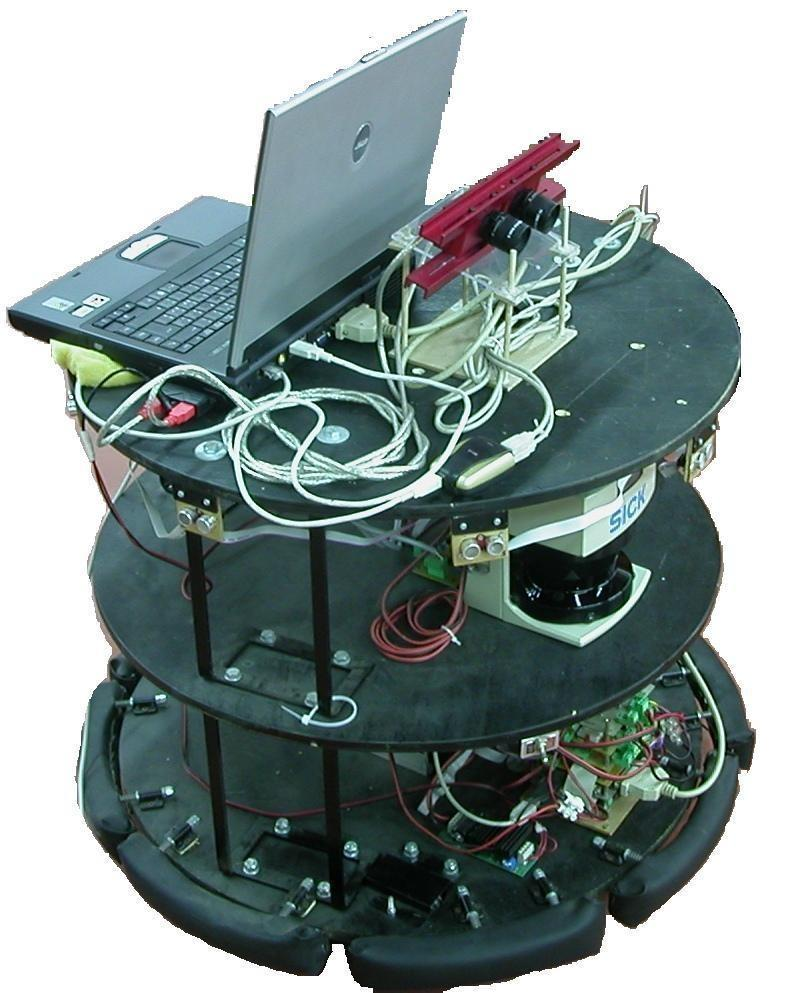
\includegraphics[width=\textwidth]{img/3morduc.jpg}
    }

    \column{0.5\textwidth}
    \visible<2-> {

      \begin{block} {\alert{\texttt{3m.o.r.d.u.c. features}}}
        
        \pause
        
        \begin{itemize}
          
          \pause
        \item \alert{\textit{mobility configuration}} \\
          differential-drive
          \pause
          
        \item \alert{\textit{sensors}} \\
          encoders, sonar, laser, bumpers, stereo-cameras
          \pause
          
        \item \alert{\textit{communication protocol}} \\
          HTTP server
          
        \end{itemize}
        
      \end{block}
      
    }

  \end{columns}
  
}
